\documentclass[11pt,a4paper]{report}

% Packages
\usepackage[utf8]{inputenc}
\usepackage[T1]{fontenc}
\usepackage[french]{babel}
\usepackage{graphicx}
\usepackage{geometry}
\usepackage{xcolor}
\usepackage{listings}
\usepackage{hyperref}
\usepackage{titlesec}
\usepackage{fancyhdr}
\usepackage{setspace}
\usepackage{tcolorbox}
\usepackage{tikz}
\usetikzlibrary{positioning,shapes,arrows.meta,shapes.geometric}
\usepackage{enumitem}
\usepackage{amsmath}
\usepackage{fontawesome5}
\usepackage{colortbl}

% Page geometry
\geometry{top=2.5cm, bottom=2.5cm, left=2.5cm, right=2.5cm, headheight=22pt}

% Define color scheme
\definecolor{primarycolor}{RGB}{41,128,185}
\definecolor{secondarycolor}{RGB}{52,152,219}
\definecolor{accentcolor}{RGB}{231,76,60}
\definecolor{darkgray}{RGB}{52,73,94}
\definecolor{lightgray}{RGB}{236,240,241}
\definecolor{codebg}{RGB}{40,44,52}
\definecolor{scalaborder}{RGB}{212,3,3}
\definecolor{psborder}{RGB}{0,94,255}
\definecolor{codecomment}{RGB}{106,153,85}
\definecolor{codestring}{RGB}{206,145,120}
\definecolor{codekeyword}{RGB}{86,156,214}

% Configure tcolorbox for better code blocks
\tcbuselibrary{listings,skins,breakable}
% Section formatting with modern design
\titleformat{\chapter}
  {\normalfont\LARGE\bfseries\color{primarycolor}}
  {\tikz[baseline=(char.base)]{\node[fill=primarycolor,circle,text=white,inner sep=3pt] (char) {\thechapter};}}
  {1em}
  {}
  [\vspace{2pt}{\titlerule[2pt]}]

\titleformat{\section}
  {\normalfont\Large\bfseries\color{secondarycolor}}
  {\thesection}
  {1em}
  {}
  [\vspace{1pt}{\color{secondarycolor}\titlerule[1.5pt]}]

\titleformat{\subsection}
  {\normalfont\large\bfseries\color{darkgray}}
  {\thesubsection}
  {1em}
  {}

\titleformat{\subsubsection}
  {\normalfont\normalsize\bfseries\color{darkgray}}
  {\thesubsubsection}
  {1em}
  {}

% Custom header and footer
\pagestyle{fancy}
\fancyhf{}
\fancyhead[L]{\small\textcolor{darkgray}{Système ERP}}
\fancyhead[R]{\small\textcolor{darkgray}{Cahier des Charges}}
\fancyfoot[C]{\small\textcolor{darkgray}{\thepage}}
\renewcommand{\headrulewidth}{0.5pt}
\renewcommand{\footrulewidth}{0.5pt}
\renewcommand{\headrule}{\hbox to\headwidth{\color{primarycolor}\leaders\hrule height \headrulewidth\hfill}}
\renewcommand{\footrule}{\hbox to\headwidth{\color{primarycolor}\leaders\hrule height \footrulewidth\hfill}}

% Hyperlink setup
\hypersetup{
    colorlinks=true,
    linkcolor=primarycolor,
    urlcolor=secondarycolor,
    citecolor=primarycolor,
    pdfborder={0 0 0}
}

% Customize itemize
\setlist[itemize]{leftmargin=*,label=\textcolor{primarycolor}{\textbullet}}



















\begin{document}

% Title page
\begin{titlepage}
    % Decorative top bar
    \tikz[remember picture,overlay]{
        \fill[primarycolor] (current page.north west) rectangle ([yshift=-1.2cm]current page.north east);
    }

    \centering
    \vspace*{1cm}

    % Logos
    \begin{minipage}{0.45\textwidth}
        \centering
        \includegraphics[height=2.8cm]{C:/Users/acer/Desktop/icons/ENSAK.png}
    \end{minipage}
    \hfill
    \begin{minipage}{0.45\textwidth}
        \centering
        \includegraphics[height=2.8cm]{C:/Users/acer/Desktop/icons/logo_harmony.png}
    \end{minipage}

    \vspace{0.6cm}
    {\color{primarycolor}\rule{\linewidth}{0.5pt}}

    \vspace{0.4cm}

    % % Institutions
    % {\large\color{darkgray} Université Sultan Moulay Slimane\\[0.15cm]}
    % {\normalsize\color{darkgray} École Nationale des Sciences Appliquées de Khouribga}
    % {}

    \vspace{0.8cm}

    % Document type
    \begin{tcolorbox}[
            enhanced,
            colback=primarycolor,
            colframe=primarycolor,
            arc=3mm,
            boxrule=0pt,
            width=0.75\textwidth,
            halign=center,
            top=8pt, bottom=8pt
        ]
        {\LARGE\bfseries\color{white} CAHIER DES CHARGES}
    \end{tcolorbox}

    \vspace{0.6cm}

    % Project title
    {\Huge\bfseries\color{darkgray} Conception et Développement d'un Système ERP\\[0.3cm]}
    {\huge\color{secondarycolor} Module Recrutement \& Gestion de Projets}

    \vspace{0.4cm}
    {\color{primarycolor}\rule{0.5\linewidth}{0.5pt}}

    \vspace{0.5cm}

    % Stage info
    {\normalsize\color{darkgray}\textbf{Stage de fin d'études}\\[0.15cm]}
    {\small\color{darkgray} Filière : Informatique et ingénierie de données}

    \vfill

    % Info table
    \begin{tcolorbox}[
            enhanced,
            colback=lightgray,
            colframe=primarycolor,
            arc=2mm,
            boxrule=0.8pt,
            width=0.9\textwidth,
            left=8pt, right=8pt, top=6pt, bottom=6pt
        ]
        \begin{tabular}{@{}p{4.5cm} p{9.5cm}@{}}
            \textbf{\color{primarycolor}Réalisé par :}         & CHERGUI Moad      \\[0.2cm]
            \textbf{\color{primarycolor}Organisme d'accueil :} & Harmony Technology \\[0.2cm]
            \textbf{\color{primarycolor}Année universitaire :} & 2025 -- 2026      \\
        \end{tabular}    \end{tcolorbox}

    \vspace{0.6cm}
    % validation and signature
    \begin{tabular}{p{6cm} p{6cm}}
        \textbf{Validé par :} & \textbf{Signature :} \\[2em]
        \hrulefill            & \hrulefill           \\
    \end{tabular}    %\end{tcolorbox}

    \vspace{0.5cm}

    % Decorative bottom bar
    \tikz[remember picture,overlay]{
        \fill[primarycolor] (current page.south west) rectangle ([yshift=0.8cm]current page.south east);
    }

\end{titlepage}

% Reset page style for content
\fancypagestyle{plain}{
    \fancyhf{}
    \fancyfoot[C]{\small\textcolor{darkgray}{\thepage}}
    \renewcommand{\headrulewidth}{0pt}
    \renewcommand{\footrulewidth}{0.5pt}
    \renewcommand{\footrule}{\hbox to\headwidth{\color{primarycolor}\leaders\hrule height \footrulewidth\hfill}}
}

\newpage
\tableofcontents
\newpage

% ============================================================
% CHAPTER 1: Contexte et Objectifs
% ============================================================
\chapter{Contexte Général et Objectifs du Projet}
% dans le cadre de mon projet de fin d'études
\section{Contexte}
Dans un environnement professionnel en constante évolution, les entreprises ont besoin d'outils intégrés pour gérer efficacement leurs ressources humaines et leurs projets. Le présent cahier des charges définit les spécifications fonctionnelles et techniques d'un \textbf{système ERP (Enterprise Resource Planning)} composé de deux modules principaux :
\begin{itemize}
    \item \textbf{Module Recrutement (Hiring)} : automatisation et optimisation du processus de recrutement grâce à l'intelligence artificielle.
    \item \textbf{Module Gestion de Projets (Project Management)} : suivi des projets, affectation des tâches et collaboration d'équipe.
\end{itemize}

\section{Objectifs du Projet}
\begin{tcolorbox}[enhanced, colback=lightgray, colframe=primarycolor, arc=3mm, boxrule=1pt, title={\color{white} Objectifs Principaux}, fonttitle=\bfseries, coltitle=white, colbacktitle=primarycolor]
    \begin{enumerate}[label=\textcolor{primarycolor}{\arabic*.}]
        \item Développer un système ERP modulaire et extensible.
        \item Automatiser le processus de recrutement, de la publication d'offres au classement des candidats par IA.
        \item Fournir un outil complet de gestion de projets avec vues Kanban et Scrum.
        \item Intégrer l'intelligence artificielle pour l'analyse de CV et la suggestion d'affectation de tâches.
        \item Offrir une interface web intuitive et responsive.
        \item Mettre en place un système de notifications en temps réel.
        \item Gamifier la gestion de projets via un système de points de récompense.
    \end{enumerate}
\end{tcolorbox}

\section{Périmètre du Projet}
Le projet couvre les deux modules suivants :
\begin{itemize}
    \item \textbf{Recrutement} : création d'offres, candidatures en ligne, stockage de CV, analyse IA, planification d'entretiens.
    \item \textbf{Gestion de Projets} : création de projets, gestion de tâches, affectation d'équipes, suivi d'avancement, notifications, système de récompenses.
\end{itemize}

% ============================================================
% CHAPTER 2: Acteurs du Système
% ============================================================
\chapter{Identification des Acteurs}

Le système interagit avec plusieurs types d'utilisateurs ayant des rôles et des permissions distincts.

\section{Acteurs Principaux}

\begin{tcolorbox}[enhanced, colback=lightgray, colframe=primarycolor, arc=3mm, boxrule=1pt]
    \begin{description}[style=nextline, font=\bfseries\color{primarycolor}]
        \item[Responsable RH (HR Manager)]
              Gère l'ensemble du processus de recrutement : création d'offres d'emploi, consultation des candidatures, examen des classements IA, et planification des entretiens.

        \item[Candidat]
              Postule aux offres d'emploi via un formulaire web et soumet son CV.

        \item[Chef de Projet (Project Manager)]
              Crée et configure les projets, assigne les tâches, ajuste les délais, et supervise l'avancement global.

        \item[Membre d'Équipe (Team Member)]
              Exécute les tâches assignées, met à jour leur statut, ajoute des commentaires, et consulte ses affectations.

        \item[Administrateur Système]
              Gère les paramètres globaux du système, les comptes utilisateurs, et les droits d'accès.
    \end{description}
\end{tcolorbox}

\section{Acteurs Secondaires}

\begin{tcolorbox}[enhanced, colback=lightgray, colframe=secondarycolor, arc=3mm, boxrule=1pt]
    \begin{description}[style=nextline, font=\bfseries\color{secondarycolor}]
        \item[Module IA]
              Composant automatisé qui analyse les CV, classe les candidats selon leurs qualifications, et suggère des affectations de tâches en fonction des compétences et de la charge de travail.

        \item[Système de Notifications]
              Service automatisé envoyant des alertes lors de mises à jour de tâches ou d'approche d'échéances.
    \end{description}
\end{tcolorbox}

% ============================================================
% CHAPTER 3: Diagrammes des Cas d'Utilisation
% ============================================================
\chapter{Diagrammes des Cas d'Utilisation}

\section{Module Recrutement}

\begin{figure}[h]
    \centering
    \begin{tikzpicture}[
            actor/.style={},
            usecase/.style={ellipse, draw=primarycolor, thick, minimum width=3cm, minimum height=1cm, align=center, fill=lightgray, font=\small},
            system/.style={rectangle, draw=secondarycolor, very thick, rounded corners},
            arrow/.style={->, >=Stealth, thick, draw=primarycolor},
            include/.style={->, >=Stealth, dashed, draw=darkgray},
        ]

        % System boundary
        \node[system, minimum width=10cm, minimum height=14cm] (system) at (5, 0) {};
        \node[above=0.1cm of system.north, font=\Large\bfseries, color=secondarycolor] {Module Recrutement};

        % Stick figure actors
        \node[actor] (hr) at (-2, 3) {
            \begin{tikzpicture}[scale=0.5]
                \draw[thick] (0,0.5) circle (0.3cm);
                \draw[thick] (0,0.2) -- (0,-0.5);
                \draw[thick] (-0.3,-0.2) -- (0.3,-0.2);
                \draw[thick] (0,-0.5) -- (-0.3,-1);
                \draw[thick] (0,-0.5) -- (0.3,-1);
                \node[below=0.8cm, font=\tiny\bfseries] at (0,-1) {Responsable RH};
            \end{tikzpicture}
        };

        \node[actor] (candidat) at (-2, -3) {
            \begin{tikzpicture}[scale=0.5]
                \draw[thick] (0,0.5) circle (0.3cm);
                \draw[thick] (0,0.2) -- (0,-0.5);
                \draw[thick] (-0.3,-0.2) -- (0.3,-0.2);
                \draw[thick] (0,-0.5) -- (-0.3,-1);
                \draw[thick] (0,-0.5) -- (0.3,-1);
                \node[below=0.8cm, font=\tiny\bfseries] at (0,-1) {Candidat};
            \end{tikzpicture}
        };

        \node[actor] (ai) at (12, 0) {
            \begin{tikzpicture}[scale=0.5]
                \draw[thick] (0,0.5) circle (0.3cm);
                \draw[thick] (0,0.2) -- (0,-0.5);
                \draw[thick] (-0.3,-0.2) -- (0.3,-0.2);
                \draw[thick] (0,-0.5) -- (-0.3,-1);
                \draw[thick] (0,-0.5) -- (0.3,-1);
                \node[below=0.8cm, font=\tiny\bfseries] at (0,-1) {Module IA};
            \end{tikzpicture}
        };

        % Use cases
        \node[usecase] (create) at (5, 5) {Créer offre\\d'emploi};
        \node[usecase] (manage) at (5, 3.5) {Gérer offres\\d'emploi};
        \node[usecase] (view) at (5, 2) {Consulter\\candidatures};
        \node[usecase] (schedule) at (5, 0.5) {Planifier\\entretiens};
        \node[usecase] (ranking) at (5, -1) {Consulter\\classement IA};
        \node[usecase] (apply) at (5, -5) {Postuler à\\une offre};
        \node[usecase] (analyze) at (5, -3) {Analyser CV};

        % Associations
        \draw[arrow] (hr) -- (create);
        \draw[arrow] (hr) -- (manage);
        \draw[arrow] (hr) -- (view);
        \draw[arrow] (hr) -- (schedule);
        \draw[arrow] (hr) -- (ranking);

        \draw[arrow] (candidat) -- (apply);
        \draw[arrow] (ai) -- (analyze);

        % Include/Extend relationships
        \draw[include] (apply) -- (analyze) node[midway, right, font=\tiny] {<<include>>};
        \draw[include] (analyze) -- (ranking) node[midway, right, font=\tiny] {<<extend>>};

    \end{tikzpicture}
    \caption{Diagramme de cas d'utilisation - Module Recrutement}
\end{figure}

\newpage

\section{Module Gestion de Projets}

\begin{figure}[h]
    \centering
    \begin{tikzpicture}[
            actor/.style={},
            usecase/.style={ellipse, draw=primarycolor, thick, minimum width=3cm, minimum height=1cm, align=center, fill=lightgray, font=\small},
            system/.style={rectangle, draw=secondarycolor, very thick, rounded corners},
            arrow/.style={->, >=Stealth, thick, draw=primarycolor},
            include/.style={->, >=Stealth, dashed, draw=darkgray},
        ]

        % System boundary
        \node[system, minimum width=10cm, minimum height=17cm] (system) at (5, 0) {};
        \node[above=0.1cm of system.north, font=\Large\bfseries, color=secondarycolor] {Module Gestion de Projets};

        % Stick figure actors
        \node[actor] (pm) at (-2, 4) {
            \begin{tikzpicture}[scale=0.5]
                \draw[thick] (0,0.5) circle (0.3cm);
                \draw[thick] (0,0.2) -- (0,-0.5);
                \draw[thick] (-0.3,-0.2) -- (0.3,-0.2);
                \draw[thick] (0,-0.5) -- (-0.3,-1);
                \draw[thick] (0,-0.5) -- (0.3,-1);
                \node[below=0.8cm, font=\tiny\bfseries] at (0,-1) {Chef de Projet};
            \end{tikzpicture}
        };

        \node[actor] (member) at (-2, -2) {
            \begin{tikzpicture}[scale=0.5]
                \draw[thick] (0,0.5) circle (0.3cm);
                \draw[thick] (0,0.2) -- (0,-0.5);
                \draw[thick] (-0.3,-0.2) -- (0.3,-0.2);
                \draw[thick] (0,-0.5) -- (-0.3,-1);
                \draw[thick] (0,-0.5) -- (0.3,-1);
                \node[below=0.8cm, font=\tiny\bfseries] at (0,-1) {Membre d'Équipe};
            \end{tikzpicture}
        };

        \node[actor] (ai) at (12, 2) {
            \begin{tikzpicture}[scale=0.5]
                \draw[thick] (0,0.5) circle (0.3cm);
                \draw[thick] (0,0.2) -- (0,-0.5);
                \draw[thick] (-0.3,-0.2) -- (0.3,-0.2);
                \draw[thick] (0,-0.5) -- (-0.3,-1);
                \draw[thick] (0,-0.5) -- (0.3,-1);
                \node[below=0.8cm, font=\tiny\bfseries] at (0,-1) {Module IA};
            \end{tikzpicture}
        };

        \node[actor] (notif) at (12, -4) {
            \begin{tikzpicture}[scale=0.5]
                \draw[thick] (0,0.5) circle (0.3cm);
                \draw[thick] (0,0.2) -- (0,-0.5);
                \draw[thick] (-0.3,-0.2) -- (0.3,-0.2);
                \draw[thick] (0,-0.5) -- (-0.3,-1);
                \draw[thick] (0,-0.5) -- (0.3,-1);
                \node[below=0.8cm, font=\tiny\bfseries] at (0,-1) {Système Notif.};
            \end{tikzpicture}
        };

        % Use cases
        \node[usecase] (createproj) at (4, 6.5) {Créer\\projet};
        \node[usecase] (createtask) at (4, 5) {Créer\\tâche};
        \node[usecase] (assign) at (5, 3.5) {Assigner\\tâches};
        \node[usecase] (suggest) at (4, 1.5) {Suggérer\\affectations};
        \node[usecase] (configure) at (4, 0) {Gérer\\projet};
        \node[usecase] (update) at (4, -3) {Mettre à jour\\statut};
        \node[usecase] (view) at (4, -1.5) {Consulter\\tâches};
        \node[usecase] (comment) at (4, -7) {Ajouter\\commentaires};
        \node[usecase] (notify) at (7, -5) {Envoyer\\notifications};

        % Associations - Chef de Projet
        \draw[arrow] (pm) -- (createproj);
        \draw[arrow] (pm) -- (createtask);
        \draw[arrow] (pm) -- (assign);
        \draw[arrow] (pm) -- (configure);
        \draw[arrow] (pm) -- (view);

        % Associations - Membre d'Équipe
        \draw[arrow] (member) -- (update);
        \draw[arrow] (member) -- (view);
        \draw[arrow] (member) -- (comment);

        % Associations - Module IA & Notifications
        \draw[arrow] (ai) -- (suggest);
        \draw[arrow] (notif) -- (notify);

        % Include/Extend relationships
        \draw[include] (suggest) -- (assign) node[midway, right, font=\tiny] {<<extend>>};
        \draw[include] (update) -- (notify) node[midway, right, font=\tiny] {<<include>>};
        \draw[include] (comment) -- (notify) node[midway, right, font=\tiny] {<<include>>};
        \draw[include] (assign) -- (notify) node[midway, right, font=\tiny] {<<include>>};

    \end{tikzpicture}
    \caption{Diagramme de cas d'utilisation - Module Gestion de Projets}
\end{figure}

% ============================================================
% CHAPTER 4: Besoins Fonctionnels
% ============================================================
\chapter{Besoins Fonctionnels}

\section{Module Recrutement (Hiring)}

\subsection{Gestion des Offres d'Emploi}
\begin{tcolorbox}[enhanced, colback=lightgray, colframe=primarycolor, arc=2mm, boxrule=0.5pt, breakable]
    \begin{itemize}
        \item Le responsable RH peut \textbf{créer des offres d'emploi} avec titre, description, compétences requises, type de contrat et date limite.
        \item Les offres peuvent être publiées, mises en pause ou clôturées.
        \item Un tableau de bord affiche l'ensemble des offres avec leur statut et le nombre de candidatures reçues.
    \end{itemize}
\end{tcolorbox}

\subsection{Candidatures en Ligne}
\begin{tcolorbox}[enhanced, colback=lightgray, colframe=primarycolor, arc=2mm, boxrule=0.5pt, breakable]
    \begin{itemize}
        \item Les candidats peuvent \textbf{postuler via un formulaire web} accessible sans authentification.
        \item Le formulaire permet de renseigner les informations personnelles, l'expérience, et de joindre un CV.
        \item Les \textbf{CV sont stockés} de manière sécurisée dans le système.
    \end{itemize}
\end{tcolorbox}

\subsection{Analyse IA des Candidatures}
\begin{tcolorbox}[enhanced, colback=lightgray, colframe=accentcolor, arc=2mm, boxrule=0.5pt, breakable, title={\color{white} Intelligence Artificielle}, fonttitle=\bfseries, coltitle=white, colbacktitle=accentcolor]
    \begin{itemize}
        \item Le module IA \textbf{analyse automatiquement les CV} soumis.
        \item Les candidats sont \textbf{classés par pertinence} en fonction de leurs qualifications par rapport au poste.
        \item Un score de compatibilité est attribué à chaque candidature.
    \end{itemize}
\end{tcolorbox}

\subsection{Sélection et Entretiens}
\begin{tcolorbox}[enhanced, colback=lightgray, colframe=primarycolor, arc=2mm, boxrule=0.5pt, breakable]
    \begin{itemize}
        \item Le responsable RH peut \textbf{consulter le classement} des candidats avec leurs scores.
        \item Il peut \textbf{planifier des entretiens} directement depuis l'interface.
        \item Le suivi du processus de recrutement est visible pour chaque offre.
    \end{itemize}
\end{tcolorbox}

\section{Module Gestion de Projets}

\subsection{Gestion des Projets}
\begin{tcolorbox}[enhanced, colback=lightgray, colframe=primarycolor, arc=2mm, boxrule=0.5pt, breakable]
    \begin{itemize}
        \item Chaque projet possède un \textbf{nom, une description, des dates de début et de fin}, et une liste de tâches.
        \item Les projets ont des \textbf{échéances (deadlines)} à respecter.
        \item Chaque tâche est \textbf{assignée à un ou plusieurs membres} de l'équipe.
    \end{itemize}
\end{tcolorbox}

\subsection{Gestion des Tâches}
\begin{tcolorbox}[enhanced, colback=lightgray, colframe=primarycolor, arc=2mm, boxrule=0.5pt, breakable]
    \begin{itemize}
        \item Affichage des tâches en \textbf{vue Kanban} et \textbf{vue Scrum}.
        \item La \textbf{vue Tâche} affiche les membres assignés à chaque tâche.
        \item La \textbf{vue Membre} affiche les tâches assignées à chaque membre de l'équipe.
        \item Les tâches peuvent être planifiées pour le \textbf{matin ou l'après-midi}.
        \item Les membres peuvent \textbf{mettre à jour le statut} des tâches et \textbf{ajouter des commentaires}.
        \item Le chef de projet peut \textbf{réassigner les tâches} et \textbf{ajuster les délais} si nécessaire.
    \end{itemize}
\end{tcolorbox}

\subsection{Suggestion IA pour l'Affectation}
\begin{tcolorbox}[enhanced, colback=lightgray, colframe=accentcolor, arc=2mm, boxrule=0.5pt, breakable, title={\color{white} Intelligence Artificielle}, fonttitle=\bfseries, coltitle=white, colbacktitle=accentcolor]
    \begin{itemize}
        \item Le système IA \textbf{suggère des affectations de tâches} en se basant sur :
              \begin{itemize}
                  \item Les \textbf{compétences} de chaque membre de l'équipe.
                  \item La \textbf{charge de travail} actuelle de chaque membre.
              \end{itemize}
        \item Le chef de projet peut accepter ou modifier les suggestions.
    \end{itemize}
\end{tcolorbox}

\subsection{Notifications}
\begin{tcolorbox}[enhanced, colback=lightgray, colframe=primarycolor, arc=2mm, boxrule=0.5pt, breakable]
    \begin{itemize}
        \item \textbf{Notifications automatiques} envoyées aux membres lorsque :
              \begin{itemize}
                  \item Une tâche est mise à jour (changement de statut, nouveau commentaire).
                  \item Une échéance approche.
                  \item Une nouvelle tâche leur est assignée.
              \end{itemize}
        \item Les notifications sont accessibles via l'interface web et par e-mail.
    \end{itemize}
\end{tcolorbox}

\subsection{Système de Récompenses}
\begin{tcolorbox}[enhanced, colback=lightgray, colframe=primarycolor, arc=2mm, boxrule=0.5pt, breakable]
    \begin{itemize}
        \item Les membres d'équipe reçoivent des \textbf{points de récompense} pour la complétion de tâches dans les délais.
        \item Un tableau de classement (leaderboard) est visible pour motiver l'équipe.
        \item Le barème de points est \textbf{configurable} par le chef de projet.
    \end{itemize}
\end{tcolorbox}

\subsection{Configuration}
\begin{tcolorbox}[enhanced, colback=lightgray, colframe=primarycolor, arc=2mm, boxrule=0.5pt, breakable]
    \begin{itemize}
        \item Le chef de projet peut \textbf{configurer} :
              \begin{itemize}
                  \item Les statuts de tâches disponibles (colonnes du Kanban).
                  \item Le système de points et récompenses.
                  \item Les rôles et permissions des membres de l'équipe.
              \end{itemize}
    \end{itemize}
\end{tcolorbox}

\subsection{Profil Utilisateur}
\begin{tcolorbox}[enhanced, colback=lightgray, colframe=primarycolor, arc=2mm, boxrule=0.5pt, breakable]
    \begin{itemize}
        \item Chaque utilisateur dispose d'une \textbf{page de profil personnalisée} affichant :
              \begin{itemize}
                  \item Ses informations personnelles (nom, email, rôle).
                  \item Son \textbf{département} d'appartenance.
                  \item Ses \textbf{compétences} sous forme de tags.
                  \item Ses \textbf{statistiques} : projets actifs, tâches terminées, tâches en cours.
                  \item Son \textbf{score de récompenses} accumulé.
              \end{itemize}
        \item L'utilisateur peut modifier ses informations (prénom, nom, email, compétences, département) directement depuis son profil.
    \end{itemize}
\end{tcolorbox}

\subsection{Gestion des Départements}
\begin{tcolorbox}[enhanced, colback=lightgray, colframe=primarycolor, arc=2mm, boxrule=0.5pt, breakable]
    \begin{itemize}
        \item Les employés sont \textbf{organisés par département}.
        \item Chaque département possède un nom et une description.
        \item Un utilisateur appartient à \textbf{un seul département} (optionnel).
        \item L'administrateur peut \textbf{créer, modifier et supprimer} des départements via l'interface d'administration.
        \item Le département est affiché sur le profil de l'utilisateur et dans les listes de membres.
    \end{itemize}
\end{tcolorbox}



% ============================================================
% CHAPTER 5: Besoins Non Fonctionnels
% ============================================================
\chapter{Besoins Non Fonctionnels}

\begin{tcolorbox}[enhanced, colback=lightgray, colframe=primarycolor, arc=3mm, boxrule=1pt, breakable]
    \begin{description}[style=nextline, font=\bfseries\color{primarycolor}]
        \item[Performance] ~\\[-2.7em]
              \begin{itemize}
                  \item Temps de réponse inférieur à 2 secondes pour les opérations courantes.
                  \item L'analyse IA des CV doit être complétée en moins de 30 secondes.
              \end{itemize}

        \item[Sécurité] ~\\[-2.7em]
              \begin{itemize}
                  \item Authentification sécurisée (JWT / OAuth2).
                  \item Contrôle d'accès basé sur les rôles.
                  \item Chiffrement des données sensibles (CV, informations personnelles).
              \end{itemize}

        \item[Scalabilité] ~\\[-2.7em]
              \begin{itemize}
                  \item Architecture modulaire permettant l'ajout de nouveaux modules ERP.
                  \item Possibilité de montée en charge horizontale.
              \end{itemize}

        \item[Ergonomie] ~\\[-2.7em]
              \begin{itemize}
                  \item Interface responsive (desktop, tablette, mobile).
                  \item Design intuitif respectant les principes UX modernes.
              \end{itemize}

        \item[Maintenabilité] ~\\[-2.7em]
            \begin{itemize}
                \item Code source documenté et versionné (Git).
                \item Tests unitaires et d'intégration.
            \end{itemize}
            \vspace{0.5cm}
    \end{description}
\end{tcolorbox}

% ============================================================
% CHAPTER 6: Architecture Technique
% ============================================================
\chapter{Architecture Technique}

\section{Architecture Globale proposée}
% image architecture
\begin{figure}[h]
    \centering
    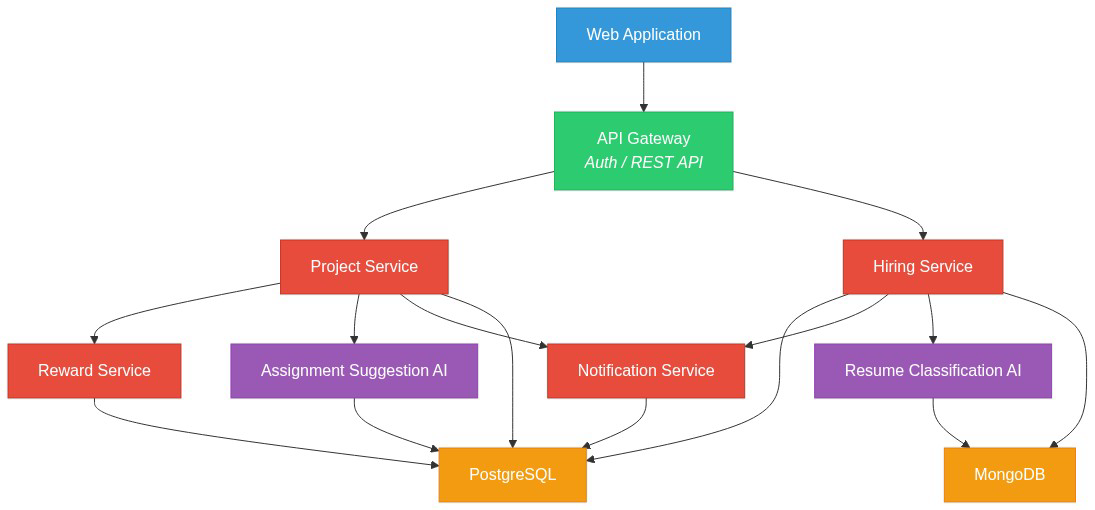
\includegraphics[width=0.8\textwidth]{imgs/architecture.png}
    \caption{Architecture Technique du Système ERP}
    % ```mermaid
    % graph TB
    %     CLIENT["Web Application"]

    %     GW["API Gateway<br/><i>Auth / REST API</i>"]

    %     HS["Hiring Service"]
    %     PS["Project Service"]
    %     NS["Notification Service"]
    %     RS["Reward Service"]

    %     CVAI["Resume Classification AI"]
    %     TAAI["Assignment Suggestion AI"]

    %     PG["PostgreSQL"]
    %     MONGO["MongoDB"]

    %     CLIENT --> GW
    %     GW --> PS
    %     GW --> HS
    %     HS --> PG
    %     HS --> NS
    %     HS --> CVAI
    %     PS --> RS
    %     PS --> TAAI
    %     PS --> NS

    %     HS --> MONGO
    %     PS --> PG
    %     CVAI --> MONGO
    %     TAAI --> PG
    %     NS --> PG
    %     RS --> PG

    %     classDef client fill:#3498db,stroke:#2980b9,color:#fff
    %     classDef gateway fill:#2ecc71,stroke:#27ae60,color:#fff
    %     classDef service fill:#e74c3c,stroke:#c0392b,color:#fff
    %     classDef ai fill:#9b59b6,stroke:#8e44ad,color:#fff
    %     classDef data fill:#f39c12,stroke:#e67e22,color:#fff

    %     class CLIENT client
    %     class GW gateway
    %     class HS,PS,NS,RS service
    %     class CVAI,TAAI ai
    %     class PG,MONGO data
    % ```
\end{figure}


\section{Stack Technologique Proposé}

\begin{tcolorbox}[enhanced, colback=lightgray, colframe=primarycolor, arc=3mm, boxrule=1pt, breakable]
    \begin{tabular}{|p{4cm}|p{9cm}|}
        \hline
        \rowcolor{primarycolor!20}
        \textbf{Couche}           & \textbf{Technologies} \\
        \hline
        Frontend                  & React.js, Htmx, vue.js, Tailwind CSS \\
        \hline
        Backend                   & Django , FastAPI \\
        \hline
        Base de données           & PostgreSQL (données relationnelles), MongoDB (CV, documents) \\
        \hline
        Intelligence Artificielle & Langchain, LLM, MCP, RAG \\
        \hline
        Notifications             & WebSocket, SMTP \\
        \hline
        Authentification          & JWT \\
        \hline
        Versionning               & Git, GitHub \\
        \hline
    \end{tabular}
\end{tcolorbox}

\end{document}
